%%   (set-keyboard-coding-system 'utf-8)
\documentclass[tikz]{standalone}
\usepackage{tikz}
\usepackage{pgfplots}
\usetikzlibrary{matrix, positioning, shapes}
\usetikzlibrary{arrows, arrows.meta, automata, shadows, patterns}

\begin{document}
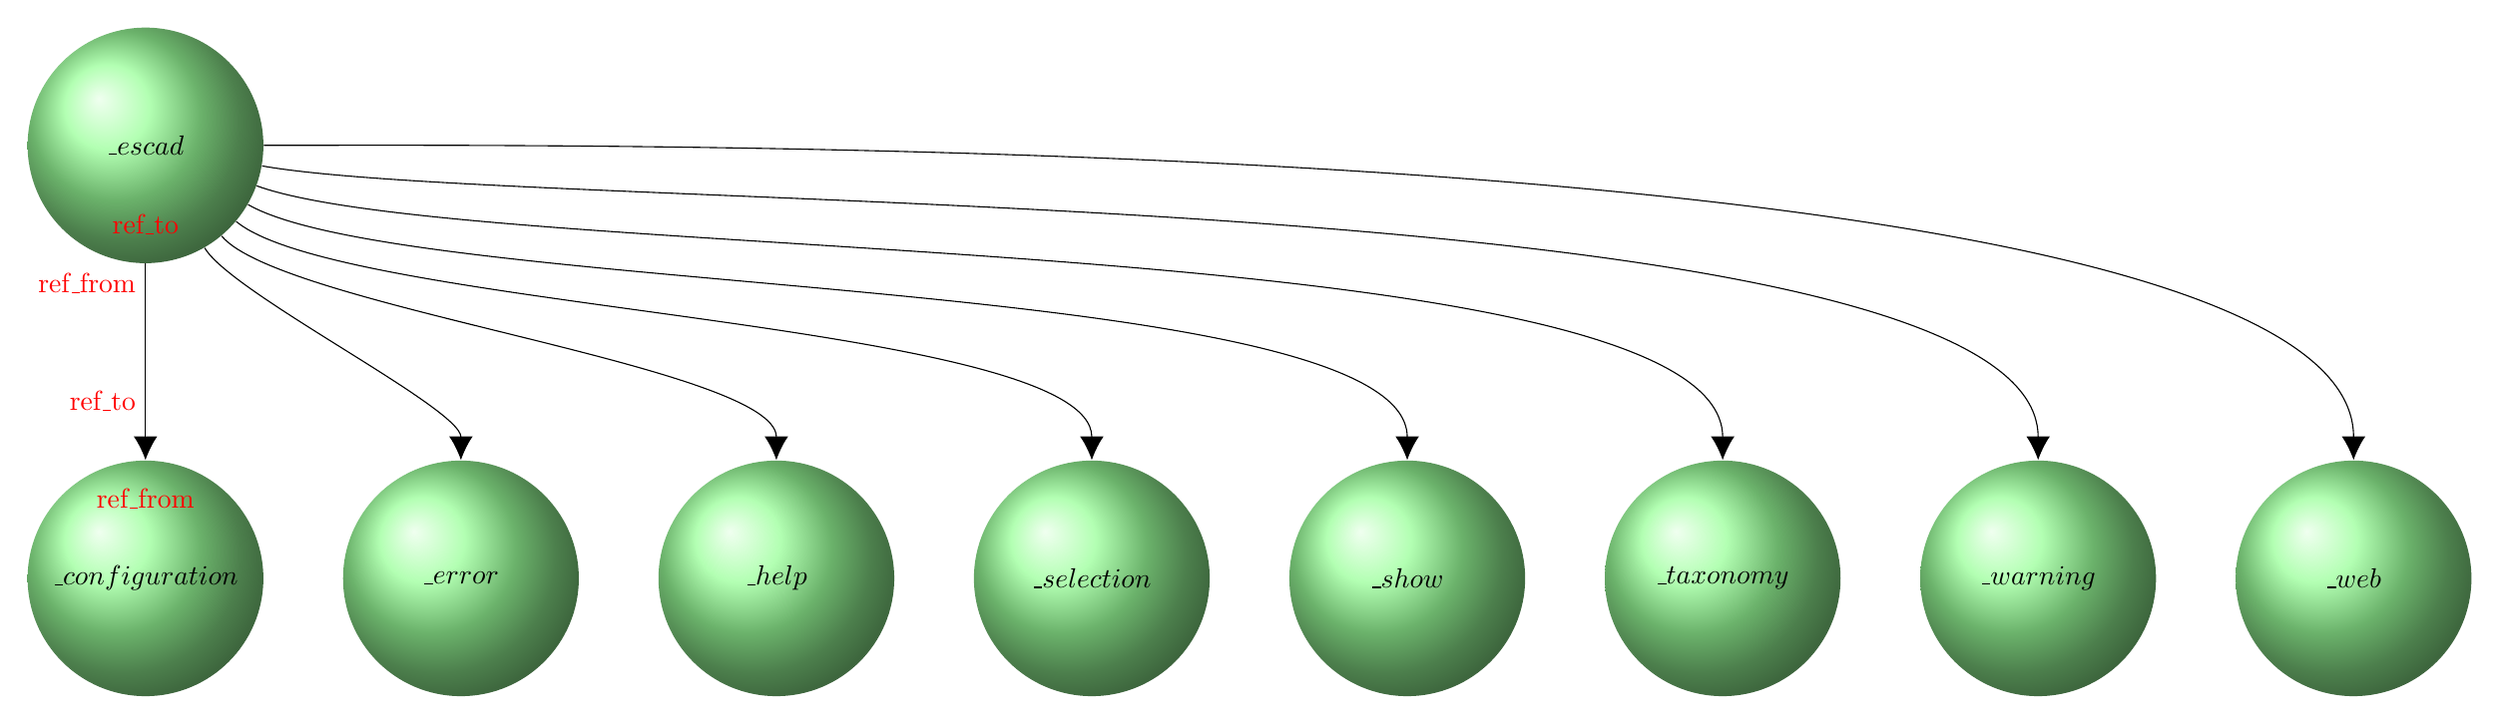
\begin{tikzpicture}[
      node distance=2.5cm and 1cm,
      sym/.style={circle, shading=ball, ball color=green!40, minimum size=30mm},
      atr/.style={circle, fill=blue!50, minimum size=0.5mm}]
      \node[sym] (escad) {$\_escad$};
      \node[sym] (configuration) [below=of escad] {$\_configuration$};
      \node[sym] (error) [right=of configuration] {$\_error$};
      \node[sym] (help) [right=of error] {$\_help$};
      \node[sym] (selection) [right=of help] {$\_selection$};
      \node[sym] (show) [right=of selection] {$\_show$};
      \node[sym] (taxonomy) [right=of show] {$\_taxonomy$};
      \node[sym] (warning) [right=of taxonomy] {$\_warning$};
      \node[sym] (web) [right=of warning] {$\_web$};

    % \node[sym] (s1) [below left=of s0] {$s_1$};
    % \node[atr] at (-1.4,-1.6) {}; % s1 attribute
    % \node[sym] (s2) [left=of s1] {$s_2$};
    % \node[sym] (s3) [left=of s2] {$s_3$};
      \draw[-{Latex[width=3mm, length=3mm]}] (escad) -- (configuration) node [pos=-0.1, above, color=red] {ref\_to} node [pos=0.1, left, color=red] {ref\_from} node [pos=0.7, left, color=red] {ref\_to} node [pos=1.1, below, color=red] {ref\_from};
      \draw[-{Latex[width=3mm, length=3mm]}] (escad) to[out=-60, in=90, looseness=0.4] (error);
      \draw[-{Latex[width=3mm, length=3mm]}] (escad) to[out=-50, in=90, looseness=0.4] (help);
      \draw[-{Latex[width=3mm, length=3mm]}] (escad) to[out=-40, in=90, looseness=0.4] (selection);
      \draw[-{Latex[width=3mm, length=3mm]}] (escad) to[out=-30, in=90, looseness=0.4] (show);
      \draw[-{Latex[width=3mm, length=3mm]}] (escad) to[out=-20, in=90, looseness=0.4] (taxonomy);
      \draw[-{Latex[width=3mm, length=3mm]}] (escad) to[out=-10, in=90, looseness=0.4] (warning);
      \draw[-{Latex[width=3mm, length=3mm]}] (escad) to[out=0, in=90, looseness=0.4] (web);
      %\draw[-{Latex[width=3mm, length=3mm]}, out=0, in=90, looseness=1] (escad) -- (web);
    % \draw[->] (s1) -- (s2) node [midway, below] {$r_1$};
    % \draw[->,out=-100,in=200,looseness=2] (s2) to node[above,pos=0.5] {$r_2$} (s3);
    % \node[atr] at (-4.9,-2.2) {}; % r2 attribute
    % \draw[->] (s3) -- (s2) node [pos=0.5, below] {$r_3$};
    % \draw[draw=black] (1,1) rectangle ++(-8,-4);
    % \node[] (view) [above=of escad] {view};
    %% legend:
    % \draw[draw=none, rounded corners=1mm, fill=yellow!40, drop shadow] (-6.9,0.9) rectangle ++(2.3,-1.4);
    % \node[sym] at (-6.5,0.6) {};
    % \node at (-5.5,0.6) {\footnotesize{symbol}};
    % \node at (-5.8,0.2) {$\leftarrow$\ \ \footnotesize{relation}};
    % \node[atr] at (-6.5,-0.2) {};
    % \node at (-5.4,-0.2) {\footnotesize{attribute}};
\end{tikzpicture}

\end{document}